\chapter{Methods III}
\label{chapter:methods III}
 
\section{Benchmarking: HBase vs MySQL}

In this section we compare our tuned HBase cluster against a standard MySQL cluster.

\bigskip

The benchmarking is based on a industry standard benchmark: Yahoo! Cloud Serving Benchmark (YCSB). For more information about this tool head to Background section: YCSB.
\par
The purpose of the benchmark is to compare HBase against MySQL in a variety of different scenarios, such as a heavy-write scenario, a heavy-read scenario, etc.
\par
YCSB works with its own data, which is represented as a table of records, each record has a unique key and an amount of fields which represent record values.
\par
Despite it does not allow users to load their own data, YCSB data is really configurable in terms of how many records user wants, how many fields has each record and the size of them. So although we can not play with the prior real data, we can almost reproduce it. Our HBase table looks really similar to the used in the whole experiment, it has the same number of fields and the size of each field is the average size of our real data fields. BloomFilters, In\_Memory and blocksize properties are enable just as in our experiments. The rest of HBase parameters looks like the ones we discussed earlier.
\par
The MySQL cluster has been compiled and subsequently deployed onto Triton with the same characteristics we have used for our HBase cluster deployment (Allocated RAM, Xeon nodes, etc). Therefore, our MySQL cluster is composed of five nodes and the data is spread evenly among them using a simple sharding function S(key), S = hash(key) \% numberOfNodes, because by default MySQL has no built-in clustering capabilities as HBase has. The MySQL table looks exactly like the HBase table does; ten fields by row, size of each one is the average size of our real data. InnoDB is used as the storage engine of our MySQL database. 
\par
\textbf{DISCLAIMER}: No MySQL-related parameters have been tuned for the benchmarks. Our MySQL cluster looks like a default deployment.

\bigskip

In the conducted benchmarks, all fields are always read, the number of operations is always one million and the records to operate on follow a uniform distribution in order to be as close as possible to our real scenario fully described in the previous chapters.



Table 7.1 summarizes the types of workload that were chosen for benchmarking.

\begin{table}[htbp]
\caption{}
\begin{tabular}{|l|r|l|l|l|}
\hline
Workload & \multicolumn{1}{l|}{ Insert \% } & Read \%  & Update \%  & Scan \% \\ \hline
Data Load  & 100 &  &  &  \\ \hline
Short range scans: workload E  & 5 &  &  & \multicolumn{1}{r|}{95} \\ \hline
Reads with heavy insert load  & 55 & \multicolumn{1}{r|}{45} &  &  \\ \hline
Scans with heavy insert load  & 55 &  &  & \multicolumn{1}{r|}{45} \\ \hline
Scans with heavy update load & \multicolumn{1}{l|}{} &  & \multicolumn{1}{r|}{55} & \multicolumn{1}{r|}{45} \\ \hline
\end{tabular}
\label{Table 1 YCSB Workloads.}
\end{table}

We run each workload from the same node, the principal one, which is the one who has the nameNode and the masterNode of Hadoop and HBase respectively.

Below we present results for each workload: load, predominant reads, reads with updates, and scans with heavy load and with heavy updates.







%http://www.pdl.cmu.edu/PDL-FTP/Storage/socc2011_abs.shtml

\subsection{Insert phase}


\begin{figure}[htb]
\centering
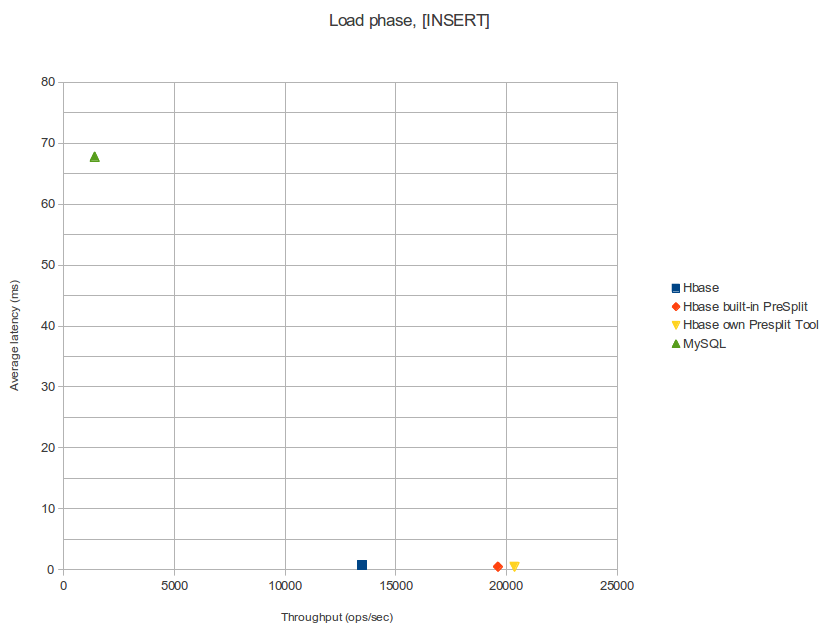
\includegraphics[width=0.7\textwidth]{./images/load.png}
 \label{fig:load}
\caption{}
\end{figure}


Along with MySQL outcome, three different versions of HBase loads are depicted due to the lack of pre-split regions YCSB comes with. The first one, \textit{HBase} label, shows the default behaviour of YCSB, which is a table with only one region at the beginning. The other two correspond to different split region algorithms we have tested. The first, \textit{HBase built-in PreSplit} label, is based on the \textit{HBase.util.RegionSplitter} tool which allows users to create tables with a specified number of pre-split regions, assuming keys are uniformly distributed bytes. This tool gives out a much better performance than the \textit{HBase} version without pre-split regions. However, this can be improved a bit more because of the fact that YCSB does not export uniformly distributed bytes keys. Instead, it creates keys which are a combination of the String \textit{user} and a Long Integer (Ex. "user111111111111111").
\par
Once we understood the YCSB key-creation, we developed a custom lightweight \textit{RegionSplitter} tool which leverages the YCSB key specification and creates a table with pre-split regions whose split points fits with the keys that YCSB will randomly create during the load phase. This tool, \textit{HBase PreSplit Tool} label, overcomes the previous results by achieving 20356 operations per second,  66.25\% better compared to the YCSB default throughput behavior (\textit{HBase} label). 
\par
We conclude that our tuned HBase cluster has unconquerable superiority in writes while MySQL is really far away from the HBase results.


\subsection{Predominant reads}



\subsection{Reads mixed with Updates}


Elasticity!!!!!!
-no digo que tengo 10 millones de records...





































